\section{Amarok::Raw\-Scope Class Reference}
\label{classAmarok_1_1RawScope}\index{Amarok::RawScope@{Amarok::RawScope}}
{\tt \#include $<$amarokarts.h$>$}

Collaboration diagram for Amarok::Raw\-Scope:\begin{figure}[H]
\begin{center}
\leavevmode
\includegraphics[width=95pt]{classAmarok_1_1RawScope__coll__graph}
\end{center}
\end{figure}
\subsection*{Public Types}
\begin{CompactItemize}
\item 
typedef {\bf Raw\-Scope\_\-base} {\bf \_\-base\_\-class}
\end{CompactItemize}
\subsection*{Public Member Functions}
\begin{CompactItemize}
\item 
{\bf Raw\-Scope} ()
\item 
{\bf Raw\-Scope} (const Arts::Sub\-Class \&s)
\item 
{\bf Raw\-Scope} (const Arts::Reference \&r)
\item 
{\bf Raw\-Scope} (const Arts::Dynamic\-Cast \&c)
\item 
{\bf Raw\-Scope} (const {\bf Raw\-Scope} \&target)
\item 
{\bf Raw\-Scope} (Arts::Object::Pool \&p)
\item 
{\bf Raw\-Scope} \& {\bf operator=} (const {\bf Raw\-Scope} \&target)
\item 
{\bf operator Arts::Stereo\-Effect} () const 
\item 
{\bf operator Arts::Synth\-Module} () const 
\item 
{\bf Raw\-Scope\_\-base} $\ast$ {\bf \_\-base} ()
\item 
Arts::Auto\-Suspend\-State {\bf auto\-Suspend} ()
\item 
void {\bf start} ()
\item 
void {\bf stop} ()
\item 
void {\bf stream\-Init} ()
\item 
void {\bf stream\-Start} ()
\item 
void {\bf stream\-End} ()
\item 
long {\bf buffer} ()
\item 
void {\bf buffer} (long \_\-new\-Value)
\item 
std::vector$<$ float $>$ $\ast$ {\bf scope} ()
\end{CompactItemize}
\subsection*{Static Public Member Functions}
\begin{CompactItemize}
\item 
{\bf Raw\-Scope} {\bf null} ()
\item 
{\bf Raw\-Scope} {\bf \_\-from\_\-base} ({\bf Raw\-Scope\_\-base} $\ast$b)
\end{CompactItemize}
\subsection*{Protected Member Functions}
\begin{CompactItemize}
\item 
{\bf Raw\-Scope} ({\bf Raw\-Scope\_\-base} $\ast$b)
\end{CompactItemize}
\subsection*{Private Member Functions}
\begin{CompactItemize}
\item 
{\bf Raw\-Scope\_\-base} $\ast$ {\bf \_\-method\_\-call} ()
\end{CompactItemize}
\subsection*{Static Private Member Functions}
\begin{CompactItemize}
\item 
Arts::Object\_\-base $\ast$ {\bf \_\-Creator} ()
\end{CompactItemize}
\subsection*{Private Attributes}
\begin{CompactItemize}
\item 
{\bf Raw\-Scope\_\-base} $\ast$ {\bf \_\-cache}
\end{CompactItemize}


\subsection{Member Typedef Documentation}
\index{Amarok::RawScope@{Amarok::Raw\-Scope}!_base_class@{\_\-base\_\-class}}
\index{_base_class@{\_\-base\_\-class}!Amarok::RawScope@{Amarok::Raw\-Scope}}
\subsubsection{\setlength{\rightskip}{0pt plus 5cm}typedef {\bf Raw\-Scope\_\-base} {\bf Amarok::Raw\-Scope::\_\-base\_\-class}}\label{classAmarok_1_1RawScope_Amarok_1_1RawScopew0}




Definition at line 205 of file amarokarts.h.

\subsection{Constructor \& Destructor Documentation}
\index{Amarok::RawScope@{Amarok::Raw\-Scope}!RawScope@{RawScope}}
\index{RawScope@{RawScope}!Amarok::RawScope@{Amarok::Raw\-Scope}}
\subsubsection{\setlength{\rightskip}{0pt plus 5cm}Amarok::Raw\-Scope::Raw\-Scope ({\bf Raw\-Scope\_\-base} $\ast$ {\em b})\hspace{0.3cm}{\tt  [inline, protected]}}\label{classAmarok_1_1RawScope_Amarok_1_1RawScopeb0}




Definition at line 201 of file amarokarts.h.



\footnotesize\begin{verbatim}201 : Arts::Object(b), _cache(0) {}
\end{verbatim}\normalsize 
\index{Amarok::RawScope@{Amarok::Raw\-Scope}!RawScope@{RawScope}}
\index{RawScope@{RawScope}!Amarok::RawScope@{Amarok::Raw\-Scope}}
\subsubsection{\setlength{\rightskip}{0pt plus 5cm}Amarok::Raw\-Scope::Raw\-Scope ()\hspace{0.3cm}{\tt  [inline]}}\label{classAmarok_1_1RawScope_Amarok_1_1RawScopea0}




Definition at line 207 of file amarokarts.h.

Referenced by \_\-from\_\-base(), and null().



\footnotesize\begin{verbatim}207 : Arts::Object(_Creator), _cache(0) {}
\end{verbatim}\normalsize 
\index{Amarok::RawScope@{Amarok::Raw\-Scope}!RawScope@{RawScope}}
\index{RawScope@{RawScope}!Amarok::RawScope@{Amarok::Raw\-Scope}}
\subsubsection{\setlength{\rightskip}{0pt plus 5cm}Amarok::Raw\-Scope::Raw\-Scope (const Arts::Sub\-Class \& {\em s})\hspace{0.3cm}{\tt  [inline]}}\label{classAmarok_1_1RawScope_Amarok_1_1RawScopea1}




Definition at line 208 of file amarokarts.h.



\footnotesize\begin{verbatim}208                                                :
209                 Arts::Object(RawScope_base::_create(s.string())), _cache(0) {}
        inline RawScope(const Arts::Reference &r) :
\end{verbatim}\normalsize 
\index{Amarok::RawScope@{Amarok::Raw\-Scope}!RawScope@{RawScope}}
\index{RawScope@{RawScope}!Amarok::RawScope@{Amarok::Raw\-Scope}}
\subsubsection{\setlength{\rightskip}{0pt plus 5cm}Amarok::Raw\-Scope::Raw\-Scope (const Arts::Reference \& {\em r})\hspace{0.3cm}{\tt  [inline]}}\label{classAmarok_1_1RawScope_Amarok_1_1RawScopea2}




Definition at line 210 of file amarokarts.h.



\footnotesize\begin{verbatim}210                                                 :
211                 Arts::Object(r.isString()?(RawScope_base::_fromString(r.string())):(RawScope_base::_fromReference(r.reference(),true))), _cache(0) {}
        inline RawScope(const Arts::DynamicCast& c) : Arts::Object(RawScope_base::_fromDynamicCast(c.object())), _cache(0) {}
\end{verbatim}\normalsize 
\index{Amarok::RawScope@{Amarok::Raw\-Scope}!RawScope@{RawScope}}
\index{RawScope@{RawScope}!Amarok::RawScope@{Amarok::Raw\-Scope}}
\subsubsection{\setlength{\rightskip}{0pt plus 5cm}Amarok::Raw\-Scope::Raw\-Scope (const Arts::Dynamic\-Cast \& {\em c})\hspace{0.3cm}{\tt  [inline]}}\label{classAmarok_1_1RawScope_Amarok_1_1RawScopea3}




Definition at line 212 of file amarokarts.h.



\footnotesize\begin{verbatim}212 : Arts::Object(RawScope_base::_fromDynamicCast(c.object())), _cache(0) {}
\end{verbatim}\normalsize 
\index{Amarok::RawScope@{Amarok::Raw\-Scope}!RawScope@{RawScope}}
\index{RawScope@{RawScope}!Amarok::RawScope@{Amarok::Raw\-Scope}}
\subsubsection{\setlength{\rightskip}{0pt plus 5cm}Amarok::Raw\-Scope::Raw\-Scope (const {\bf Raw\-Scope} \& {\em target})\hspace{0.3cm}{\tt  [inline]}}\label{classAmarok_1_1RawScope_Amarok_1_1RawScopea4}




Definition at line 213 of file amarokarts.h.



\footnotesize\begin{verbatim}213 : Arts::Object(target._pool), _cache(target._cache) {}
\end{verbatim}\normalsize 
\index{Amarok::RawScope@{Amarok::Raw\-Scope}!RawScope@{RawScope}}
\index{RawScope@{RawScope}!Amarok::RawScope@{Amarok::Raw\-Scope}}
\subsubsection{\setlength{\rightskip}{0pt plus 5cm}Amarok::Raw\-Scope::Raw\-Scope (Arts::Object::Pool \& {\em p})\hspace{0.3cm}{\tt  [inline]}}\label{classAmarok_1_1RawScope_Amarok_1_1RawScopea5}




Definition at line 214 of file amarokarts.h.



\footnotesize\begin{verbatim}214 : Arts::Object(p), _cache(0) {}
\end{verbatim}\normalsize 


\subsection{Member Function Documentation}
\index{Amarok::RawScope@{Amarok::Raw\-Scope}!_base@{\_\-base}}
\index{_base@{\_\-base}!Amarok::RawScope@{Amarok::Raw\-Scope}}
\subsubsection{\setlength{\rightskip}{0pt plus 5cm}{\bf Raw\-Scope\_\-base}$\ast$ Amarok::Raw\-Scope::\_\-base ()\hspace{0.3cm}{\tt  [inline]}}\label{classAmarok_1_1RawScope_Amarok_1_1RawScopea9}




Definition at line 227 of file amarokarts.h.



\footnotesize\begin{verbatim}227 {return _cache?_cache:_method_call();}
\end{verbatim}\normalsize 
\index{Amarok::RawScope@{Amarok::Raw\-Scope}!_Creator@{\_\-Creator}}
\index{_Creator@{\_\-Creator}!Amarok::RawScope@{Amarok::Raw\-Scope}}
\subsubsection{\setlength{\rightskip}{0pt plus 5cm}Arts::Object\_\-base $\ast$ Amarok::Raw\-Scope::\_\-Creator ()\hspace{0.3cm}{\tt  [static, private]}}\label{classAmarok_1_1RawScope_Amarok_1_1RawScopeh0}




Definition at line 377 of file amarokarts.cc.

References Amarok::Raw\-Scope\_\-base::\_\-create().



\footnotesize\begin{verbatim}377                                           {
378         return Amarok::RawScope_base::_create();
379 }
\end{verbatim}\normalsize 


Here is the call graph for this function:\begin{figure}[H]
\begin{center}
\leavevmode
\includegraphics[width=197pt]{classAmarok_1_1RawScope_Amarok_1_1RawScopeh0_cgraph}
\end{center}
\end{figure}
\index{Amarok::RawScope@{Amarok::Raw\-Scope}!_from_base@{\_\-from\_\-base}}
\index{_from_base@{\_\-from\_\-base}!Amarok::RawScope@{Amarok::Raw\-Scope}}
\subsubsection{\setlength{\rightskip}{0pt plus 5cm}{\bf Raw\-Scope} Amarok::Raw\-Scope::\_\-from\_\-base ({\bf Raw\-Scope\_\-base} $\ast$ {\em b})\hspace{0.3cm}{\tt  [inline, static]}}\label{classAmarok_1_1RawScope_Amarok_1_1RawScopee1}




Definition at line 216 of file amarokarts.h.

References Raw\-Scope().



\footnotesize\begin{verbatim}216 {return RawScope(b);}
\end{verbatim}\normalsize 


Here is the call graph for this function:\begin{figure}[H]
\begin{center}
\leavevmode
\includegraphics[width=198pt]{classAmarok_1_1RawScope_Amarok_1_1RawScopee1_cgraph}
\end{center}
\end{figure}
\index{Amarok::RawScope@{Amarok::Raw\-Scope}!_method_call@{\_\-method\_\-call}}
\index{_method_call@{\_\-method\_\-call}!Amarok::RawScope@{Amarok::Raw\-Scope}}
\subsubsection{\setlength{\rightskip}{0pt plus 5cm}{\bf Raw\-Scope\_\-base}$\ast$ Amarok::Raw\-Scope::\_\-method\_\-call ()\hspace{0.3cm}{\tt  [inline, private]}}\label{classAmarok_1_1RawScope_Amarok_1_1RawScoped0}




Definition at line 191 of file amarokarts.h.

References Amarok::Raw\-Scope\_\-base::\_\-cast().

Referenced by auto\-Suspend(), buffer(), scope(), start(), stop(), stream\-End(), stream\-Init(), and stream\-Start().



\footnotesize\begin{verbatim}191                                              {
192                 _pool->checkcreate();
193                 if(_pool->base) {
194                         _cache=(RawScope_base *)_pool->base->_cast(RawScope_base::_IID);
195                         assert(_cache);
196                 }
197                 return _cache;
198         }
\end{verbatim}\normalsize 


Here is the call graph for this function:\begin{figure}[H]
\begin{center}
\leavevmode
\includegraphics[width=204pt]{classAmarok_1_1RawScope_Amarok_1_1RawScoped0_cgraph}
\end{center}
\end{figure}
\index{Amarok::RawScope@{Amarok::Raw\-Scope}!autoSuspend@{autoSuspend}}
\index{autoSuspend@{autoSuspend}!Amarok::RawScope@{Amarok::Raw\-Scope}}
\subsubsection{\setlength{\rightskip}{0pt plus 5cm}Arts::Auto\-Suspend\-State Amarok::Raw\-Scope::auto\-Suspend ()\hspace{0.3cm}{\tt  [inline]}}\label{classAmarok_1_1RawScope_Amarok_1_1RawScopea10}




Definition at line 283 of file amarokarts.h.

References \_\-method\_\-call().



\footnotesize\begin{verbatim}284 {
285         return _cache?static_cast<Arts::SynthModule_base*>(_cache)->autoSuspend():static_cast<Arts::SynthModule_base*>(_method_call())->autoSuspend();
286 }
\end{verbatim}\normalsize 


Here is the call graph for this function:\begin{figure}[H]
\begin{center}
\leavevmode
\includegraphics[width=307pt]{classAmarok_1_1RawScope_Amarok_1_1RawScopea10_cgraph}
\end{center}
\end{figure}
\index{Amarok::RawScope@{Amarok::Raw\-Scope}!buffer@{buffer}}
\index{buffer@{buffer}!Amarok::RawScope@{Amarok::Raw\-Scope}}
\subsubsection{\setlength{\rightskip}{0pt plus 5cm}void Amarok::Raw\-Scope::buffer (long {\em \_\-new\-Value})\hspace{0.3cm}{\tt  [inline]}}\label{classAmarok_1_1RawScope_Amarok_1_1RawScopea17}




Definition at line 318 of file amarokarts.h.

References \_\-method\_\-call(), and Amarok::Raw\-Scope\_\-base::buffer().



\footnotesize\begin{verbatim}319 {
320          _cache?static_cast<Amarok::RawScope_base*>(_cache)->buffer(_newValue):static_cast<Amarok::RawScope_base*>(_method_call())->buffer(_newValue);
321 }
\end{verbatim}\normalsize 


Here is the call graph for this function:\begin{figure}[H]
\begin{center}
\leavevmode
\includegraphics[width=291pt]{classAmarok_1_1RawScope_Amarok_1_1RawScopea17_cgraph}
\end{center}
\end{figure}
\index{Amarok::RawScope@{Amarok::Raw\-Scope}!buffer@{buffer}}
\index{buffer@{buffer}!Amarok::RawScope@{Amarok::Raw\-Scope}}
\subsubsection{\setlength{\rightskip}{0pt plus 5cm}long Amarok::Raw\-Scope::buffer ()\hspace{0.3cm}{\tt  [inline]}}\label{classAmarok_1_1RawScope_Amarok_1_1RawScopea16}




Definition at line 313 of file amarokarts.h.

References \_\-method\_\-call(), and Amarok::Raw\-Scope\_\-base::buffer().

Referenced by Arts\-Engine::init().



\footnotesize\begin{verbatim}314 {
315         return _cache?static_cast<Amarok::RawScope_base*>(_cache)->buffer():static_cast<Amarok::RawScope_base*>(_method_call())->buffer();
316 }
\end{verbatim}\normalsize 


Here is the call graph for this function:\begin{figure}[H]
\begin{center}
\leavevmode
\includegraphics[width=291pt]{classAmarok_1_1RawScope_Amarok_1_1RawScopea16_cgraph}
\end{center}
\end{figure}
\index{Amarok::RawScope@{Amarok::Raw\-Scope}!null@{null}}
\index{null@{null}!Amarok::RawScope@{Amarok::Raw\-Scope}}
\subsubsection{\setlength{\rightskip}{0pt plus 5cm}{\bf Raw\-Scope} Amarok::Raw\-Scope::null ()\hspace{0.3cm}{\tt  [inline, static]}}\label{classAmarok_1_1RawScope_Amarok_1_1RawScopee0}




Definition at line 215 of file amarokarts.h.

References Raw\-Scope().

Referenced by Arts\-Engine::$\sim$Arts\-Engine().



\footnotesize\begin{verbatim}215 {return RawScope((RawScope_base*)0);}
\end{verbatim}\normalsize 


Here is the call graph for this function:\begin{figure}[H]
\begin{center}
\leavevmode
\includegraphics[width=180pt]{classAmarok_1_1RawScope_Amarok_1_1RawScopee0_cgraph}
\end{center}
\end{figure}
\index{Amarok::RawScope@{Amarok::Raw\-Scope}!operator Arts::StereoEffect@{operator Arts::StereoEffect}}
\index{operator Arts::StereoEffect@{operator Arts::StereoEffect}!Amarok::RawScope@{Amarok::Raw\-Scope}}
\subsubsection{\setlength{\rightskip}{0pt plus 5cm}Amarok::Raw\-Scope::operator Arts::Stereo\-Effect () const\hspace{0.3cm}{\tt  [inline]}}\label{classAmarok_1_1RawScope_Amarok_1_1RawScopea7}




Definition at line 225 of file amarokarts.h.

References operator Arts::Stereo\-Effect().

Referenced by operator Arts::Stereo\-Effect().



\footnotesize\begin{verbatim}225 { return Arts::StereoEffect(*_pool); }
\end{verbatim}\normalsize 


Here is the call graph for this function:\begin{figure}[H]
\begin{center}
\leavevmode
\includegraphics[width=102pt]{classAmarok_1_1RawScope_Amarok_1_1RawScopea7_cgraph}
\end{center}
\end{figure}
\index{Amarok::RawScope@{Amarok::Raw\-Scope}!operator Arts::SynthModule@{operator Arts::SynthModule}}
\index{operator Arts::SynthModule@{operator Arts::SynthModule}!Amarok::RawScope@{Amarok::Raw\-Scope}}
\subsubsection{\setlength{\rightskip}{0pt plus 5cm}Amarok::Raw\-Scope::operator Arts::Synth\-Module () const\hspace{0.3cm}{\tt  [inline]}}\label{classAmarok_1_1RawScope_Amarok_1_1RawScopea8}




Definition at line 226 of file amarokarts.h.



\footnotesize\begin{verbatim}226 { return Arts::SynthModule(*_pool); }
\end{verbatim}\normalsize 
\index{Amarok::RawScope@{Amarok::Raw\-Scope}!operator=@{operator=}}
\index{operator=@{operator=}!Amarok::RawScope@{Amarok::Raw\-Scope}}
\subsubsection{\setlength{\rightskip}{0pt plus 5cm}{\bf Raw\-Scope}\& Amarok::Raw\-Scope::operator= (const {\bf Raw\-Scope} \& {\em target})\hspace{0.3cm}{\tt  [inline]}}\label{classAmarok_1_1RawScope_Amarok_1_1RawScopea6}




Definition at line 217 of file amarokarts.h.

References \_\-cache.



\footnotesize\begin{verbatim}217                                                            {
218                 if (_pool == target._pool) return *this;
219                 _pool->Dec();
220                 _pool = target._pool;
221                 _cache = target._cache;
222                 _pool->Inc();
223                 return *this;
224         }
\end{verbatim}\normalsize 
\index{Amarok::RawScope@{Amarok::Raw\-Scope}!scope@{scope}}
\index{scope@{scope}!Amarok::RawScope@{Amarok::Raw\-Scope}}
\subsubsection{\setlength{\rightskip}{0pt plus 5cm}std::vector$<$ float $>$ $\ast$ Amarok::Raw\-Scope::scope ()\hspace{0.3cm}{\tt  [inline]}}\label{classAmarok_1_1RawScope_Amarok_1_1RawScopea18}




Definition at line 323 of file amarokarts.h.

References \_\-method\_\-call(), and Amarok::Raw\-Scope\_\-base::scope().

Referenced by Arts\-Engine::scope().



\footnotesize\begin{verbatim}324 {
325         return _cache?static_cast<Amarok::RawScope_base*>(_cache)->scope():static_cast<Amarok::RawScope_base*>(_method_call())->scope();
326 }
\end{verbatim}\normalsize 


Here is the call graph for this function:\begin{figure}[H]
\begin{center}
\leavevmode
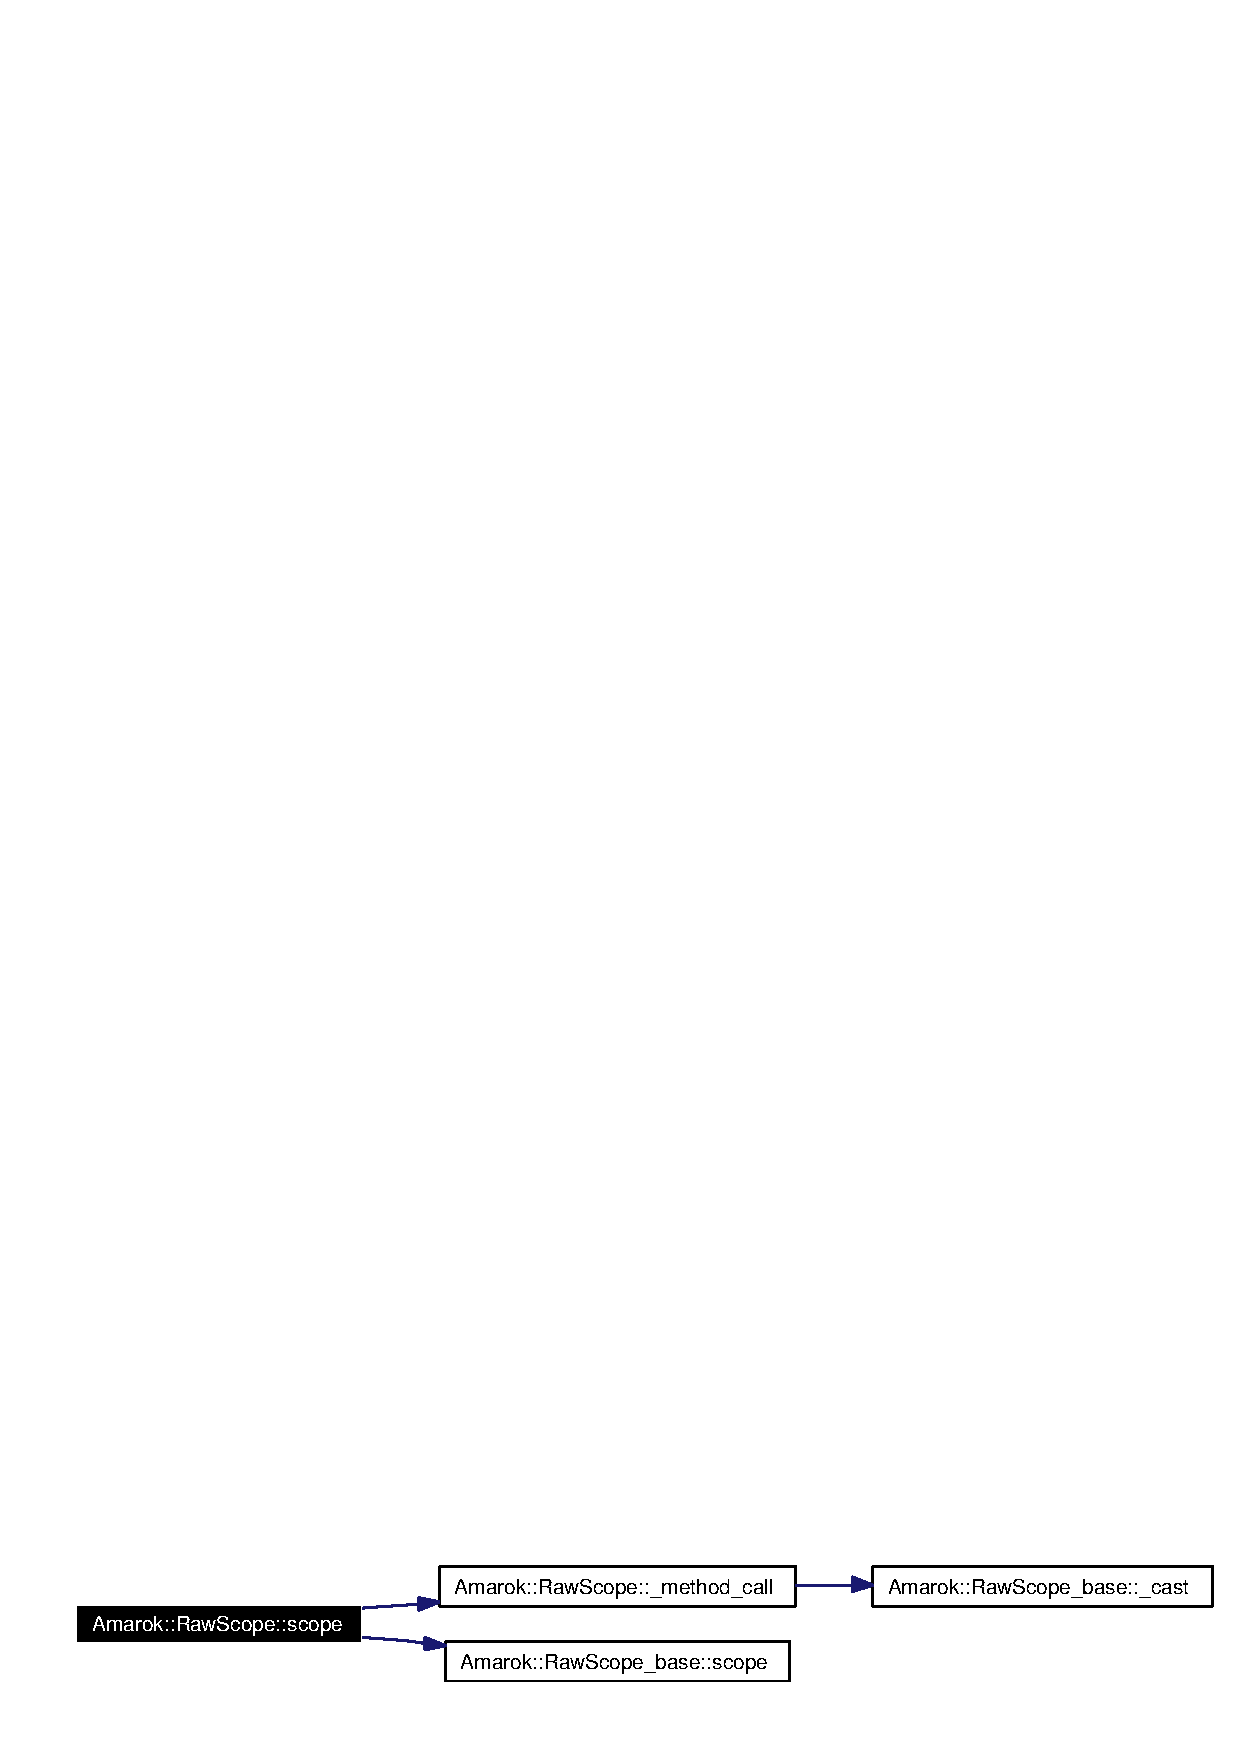
\includegraphics[width=291pt]{classAmarok_1_1RawScope_Amarok_1_1RawScopea18_cgraph}
\end{center}
\end{figure}
\index{Amarok::RawScope@{Amarok::Raw\-Scope}!start@{start}}
\index{start@{start}!Amarok::RawScope@{Amarok::Raw\-Scope}}
\subsubsection{\setlength{\rightskip}{0pt plus 5cm}void Amarok::Raw\-Scope::start ()\hspace{0.3cm}{\tt  [inline]}}\label{classAmarok_1_1RawScope_Amarok_1_1RawScopea11}




Definition at line 288 of file amarokarts.h.

References \_\-method\_\-call().

Referenced by Arts\-Engine::init().



\footnotesize\begin{verbatim}289 {
290          _cache?static_cast<Arts::SynthModule_base*>(_cache)->start():static_cast<Arts::SynthModule_base*>(_method_call())->start();
291 }
\end{verbatim}\normalsize 


Here is the call graph for this function:\begin{figure}[H]
\begin{center}
\leavevmode
\includegraphics[width=288pt]{classAmarok_1_1RawScope_Amarok_1_1RawScopea11_cgraph}
\end{center}
\end{figure}
\index{Amarok::RawScope@{Amarok::Raw\-Scope}!stop@{stop}}
\index{stop@{stop}!Amarok::RawScope@{Amarok::Raw\-Scope}}
\subsubsection{\setlength{\rightskip}{0pt plus 5cm}void Amarok::Raw\-Scope::stop ()\hspace{0.3cm}{\tt  [inline]}}\label{classAmarok_1_1RawScope_Amarok_1_1RawScopea12}




Definition at line 293 of file amarokarts.h.

References \_\-method\_\-call().



\footnotesize\begin{verbatim}294 {
295          _cache?static_cast<Arts::SynthModule_base*>(_cache)->stop():static_cast<Arts::SynthModule_base*>(_method_call())->stop();
296 }
\end{verbatim}\normalsize 


Here is the call graph for this function:\begin{figure}[H]
\begin{center}
\leavevmode
\includegraphics[width=287pt]{classAmarok_1_1RawScope_Amarok_1_1RawScopea12_cgraph}
\end{center}
\end{figure}
\index{Amarok::RawScope@{Amarok::Raw\-Scope}!streamEnd@{streamEnd}}
\index{streamEnd@{streamEnd}!Amarok::RawScope@{Amarok::Raw\-Scope}}
\subsubsection{\setlength{\rightskip}{0pt plus 5cm}void Amarok::Raw\-Scope::stream\-End ()\hspace{0.3cm}{\tt  [inline]}}\label{classAmarok_1_1RawScope_Amarok_1_1RawScopea15}




Definition at line 308 of file amarokarts.h.

References \_\-method\_\-call().



\footnotesize\begin{verbatim}309 {
310          _cache?static_cast<Arts::SynthModule_base*>(_cache)->streamEnd():static_cast<Arts::SynthModule_base*>(_method_call())->streamEnd();
311 }
\end{verbatim}\normalsize 


Here is the call graph for this function:\begin{figure}[H]
\begin{center}
\leavevmode
\includegraphics[width=302pt]{classAmarok_1_1RawScope_Amarok_1_1RawScopea15_cgraph}
\end{center}
\end{figure}
\index{Amarok::RawScope@{Amarok::Raw\-Scope}!streamInit@{streamInit}}
\index{streamInit@{streamInit}!Amarok::RawScope@{Amarok::Raw\-Scope}}
\subsubsection{\setlength{\rightskip}{0pt plus 5cm}void Amarok::Raw\-Scope::stream\-Init ()\hspace{0.3cm}{\tt  [inline]}}\label{classAmarok_1_1RawScope_Amarok_1_1RawScopea13}




Definition at line 298 of file amarokarts.h.

References \_\-method\_\-call().



\footnotesize\begin{verbatim}299 {
300          _cache?static_cast<Arts::SynthModule_base*>(_cache)->streamInit():static_cast<Arts::SynthModule_base*>(_method_call())->streamInit();
301 }
\end{verbatim}\normalsize 


Here is the call graph for this function:\begin{figure}[H]
\begin{center}
\leavevmode
\includegraphics[width=300pt]{classAmarok_1_1RawScope_Amarok_1_1RawScopea13_cgraph}
\end{center}
\end{figure}
\index{Amarok::RawScope@{Amarok::Raw\-Scope}!streamStart@{streamStart}}
\index{streamStart@{streamStart}!Amarok::RawScope@{Amarok::Raw\-Scope}}
\subsubsection{\setlength{\rightskip}{0pt plus 5cm}void Amarok::Raw\-Scope::stream\-Start ()\hspace{0.3cm}{\tt  [inline]}}\label{classAmarok_1_1RawScope_Amarok_1_1RawScopea14}




Definition at line 303 of file amarokarts.h.

References \_\-method\_\-call().



\footnotesize\begin{verbatim}304 {
305          _cache?static_cast<Arts::SynthModule_base*>(_cache)->streamStart():static_cast<Arts::SynthModule_base*>(_method_call())->streamStart();
306 }
\end{verbatim}\normalsize 


Here is the call graph for this function:\begin{figure}[H]
\begin{center}
\leavevmode
\includegraphics[width=304pt]{classAmarok_1_1RawScope_Amarok_1_1RawScopea14_cgraph}
\end{center}
\end{figure}


\subsection{Member Data Documentation}
\index{Amarok::RawScope@{Amarok::Raw\-Scope}!_cache@{\_\-cache}}
\index{_cache@{\_\-cache}!Amarok::RawScope@{Amarok::Raw\-Scope}}
\subsubsection{\setlength{\rightskip}{0pt plus 5cm}{\bf Raw\-Scope\_\-base}$\ast$ {\bf Amarok::Raw\-Scope::\_\-cache}\hspace{0.3cm}{\tt  [private]}}\label{classAmarok_1_1RawScope_Amarok_1_1RawScoper0}




Definition at line 190 of file amarokarts.h.

Referenced by operator=().

The documentation for this class was generated from the following files:\begin{CompactItemize}
\item 
{\bf amarokarts.h}\item 
{\bf amarokarts.cc}\end{CompactItemize}
